%XXX Fragile: tabulars are only the same widths because each cell is 1 \tt
%    character wide

\centering

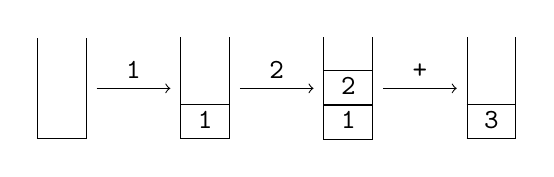
\begin{tikzpicture}[node distance=0.15\linewidth]
  \node (a) {
    \begin{tabular}{|c|}
      \texttt{~} \\
      \texttt{~} \\
      \texttt{~} \\ \hline
    \end{tabular}
  };

  \node (b) [right of=a] {
    \begin{tabular}{|c|}
      \texttt{~} \\
      \texttt{~} \\ \hline
      \texttt{1} \\ \hline
    \end{tabular}
  };

  \node (c) [right of=b] {
    \begin{tabular}{|c|}
      \texttt{~} \\ \hline
      \texttt{2} \\ \hline
      \texttt{1} \\ \hline
    \end{tabular}
  };

  \node (d) [right of=c] {
    \begin{tabular}{|c|}
      \texttt{~} \\
      \texttt{~} \\ \hline
      \texttt{3} \\ \hline
    \end{tabular}
  };

  \path[->] (a) edge node [above] {\texttt{1}} (b)
            (b) edge node [above] {\texttt{2}} (c)
            (c) edge node [above] {\texttt{+}} (d);
\end{tikzpicture}

\caption{Visualizing stack-based calculation}
